\chapter{Design Study: Interactive exploration of 3D scanned baggage} % Main chapter title
\label{DesignStudy}

\section{Introduction}
Volumetric data found in many fields, such as engineering, material sciences, medical imaging, astrophysics. Their exploration is not trivial, and heavily impacted by the users' needs. In most airports, security agents deal with such data exploration during baggage inspections. They use two types of fluoroscopic systems: X-ray and tomography scanning systems. X-ray system provides a flattened 2D baggage scan while tomography scanning system produces transversal scans, also called slices. 
Thanks to data processing (e.g. \cite{deans2007radon}), they can produce a full 3D scan (set of voxel with their corresponding density).
Our input data is a uniformly sampled multivariate field F : D $\longrightarrow$ V, D $\subset \mathbb{R}^{n}$ 
,V $\subset \mathbb{R}^{m}$ with n = 3 (volume) and m=1 (scalar field).



\section{Activity analysis}

During this thesis, I had the opportunity to intend to training courses for security agents' instructors, and to visit an airport (Toulouse-Blagnac Airport). These helped me to study the activity of security agents and get the users' needs. The training courses lasted 3 weeks. In fact, I studied weapons and Explosives, scan analysis methods, dissimulation techniques, and fluoroscopic systems functionalities. In addition, I spent 3 days among the security agents of Brink's at Toulouse-Blagnac Airport. In this section, first I describe the security agents' task by describing their equipment, the prohibited articles, and the protocol to analyze a scan. Next, I highlight their activity issues by showing the different error types, and the dissimulation techniques.

\subsection{Task description}

The airport security agents have many roles depending on their work position. They control people (the passengers, the flight crew, and the airport personnel), and the luggage at security checkpoints. The different work positions are:
\begin{itemize}
\item The reception, where the security agents check the documents and put the hand luggage on the treadmill of the X-ray machine,
\item viewing and detection of objects and luggage through X-rays,
\item pat-down search,
\item baggage inspection.
\end{itemize}
In this study, we focus on the threat detection through X-rays.

\subsubsection{The Equipment}

In most French airport, the security agents two types of fluoroscopic system: the tomograph, and the classic system. The classic fluoroscopic system provides a 2D scan of luggage on the one hand, and on the other, the tomograph can produce transversal scans in addition to the 2D scan. Some scanners are able to detect explosive automatically, they are called EDS (Explosive Detection System). The architecture of the classic system is composed of:
\begin{itemize}
\item a mechanical set comprising a frame, a conveyor, and a collimator,
\item a physical set comprising an x-ray generator, a detector, and detection cells,
\item the central unit,
\item and input/output devices (keyboard, screens).
\end{itemize}
When a luggage get in the frame, the x-rays are sent from the generator to the L-shaped detector through the luggage's components. The x-rays are attenuated depending on the molecular density of the encountered objects, which allows to receive different x-ray intensities on the L-shaped detector. Then, the different received intensities are processed to get the final 2D scan.
The final image does not keep the original colors, instead they use 3 colors (orange, green, and blue) to show the density of each encountered object. The orange color is used for low density matters which are mainly organic. In opposition, the blue color is used for high density matters which are mainly inorganic. The green color expresses the superposition of different kinds of materials or average density materials, see \ref{f:image2d}.

\begin{figure}
\centering
	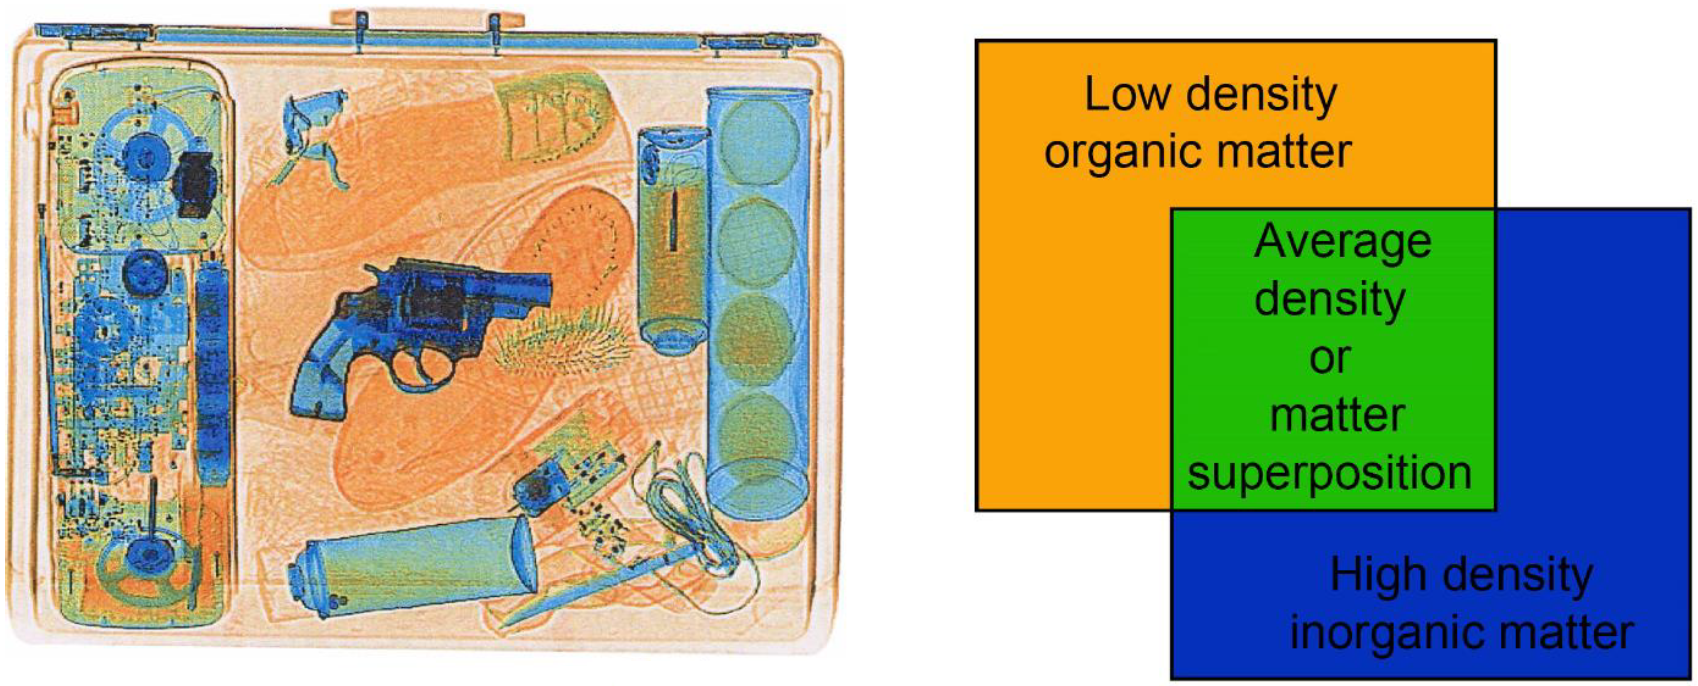
\includegraphics[height=5.2cm]{Figures/contour}
	\caption{ X-ray scan with the 3 standard colors (orange, green, and blue)}
	\label{f:image2d}
\end{figure}

\subsubsection{Prohibited articles}
Depending on the context, there are many prohibited articles. The aim is to avoid any kind of weapon to board in the aircraft. According to the regulations, weapons are items intended primarily to kill, injure, immobilize or reduce to impotence. The prohibited articles are:
\begin{itemize}
\item Guns, firearms, and any other equipment emitting projectiles,
\item Stun devices,
\item objects with a sharp tip or a cutting edge,
\item working tools,
\item blunt instruments,
\item explosive or incendiary substances and devices.
\end{itemize}
In addition to these prohibitions, some articles such as liquid, gels, and aerosols are restricted.

\subsubsection{Scan analysis}
Whatever fluoroscopic system is used, the security agents try to follow an analysis protocol to ensure any prohibited article is detected. This protocol is composed of 4 major steps, which are the global picture analysis, the in-depth analysis, the structure analysis, and the context.

\paragraph{Global picture analysis}:


First, the security agent check whether the luggage is well placed. Indeed, the luggage should appear on the screen with \ang{45} of rotation. If it is not the case, a re-positioning is required. To avoid this issue, another agent must check the luggage positioning.
Next, the agent try to find out whether the luggage is complex or not. A luggage is complex when there is a superposition of usual objects and metallic materials. A complex luggage can hide threat and make them invisible. If possible, the complex luggage is opened and all troublesome objects are removed.

\paragraph{The in-depth analysis}:


First, the security agent divides the luggage's component in groups. The aim is to reduce the risk of error. Indeed, smaller prohibited articles may be easily unseen. Then, the dark areas must be lightened up. To do it, the security agent can use functionalities such as high penetration or contour enhancement. If the area is still dark, the luggage must be opened to remove the serious doubts.
Next, the agent focus on the problematical shapes. A non-recognizable shape may be caused by a bad positioning. Any unrecognized object must be inspected by the agent. If any prohibited article is detected, the agent follows the procedure related to the threat. In addition, an organic matter superposed to an electronic device is considered as a sufficient reason to open the luggage. Liquids, gels, and aerosols should be less than 100ml otherwise they will be removed from the luggage. These liquids should be placed into a plastic bag.

\paragraph{The structure analysis}:


During this step, the security agent compare each element of the luggage which must be symmetrical because of its industrial conception such us suitcase's wheels. If the symmetry is not respected, it is might be a clue to the deliberate luggage modification for dissimulating prohibited objects.

\paragraph{The context}:


Depending on the context some articles are prohibited or not. The agent must be aware of his work position.
On an explosive detection system, the threats are already highlighted. The agent's job is to verify whether the threats are real or not.
In our study, we focus on a conventional system to provide new interaction techniques for analyzing 3D luggage scans.

\subsection{The activity issues}
There is many level of security in luggage inspection depending on the airport (between 1 and 6). Humans and machines work together to detect any potential threat inside the luggage. At the lowest levels of security, the security agents are in contact with the passengers, and therefore face 4 main operational constraints for safety and economical reasons: Facilitation, security, speed, and self-protection. 

First of all, The facilitation constraint implies that the security agent has to ensure a good user experience to the customers (the passengers). Second, they must prevent any potential threat to pass their inspection. In addition, they have to protect themselves from different kind of threats (ill-intentioned persons, parcel bomb). And finally, economical reasons oblige them to be fast enough in order to ensure a good flow. Therefore, the security agent face a trade-off between these four constraints, see figure \ref{f:constraints} .
\begin{figure}
\centering
	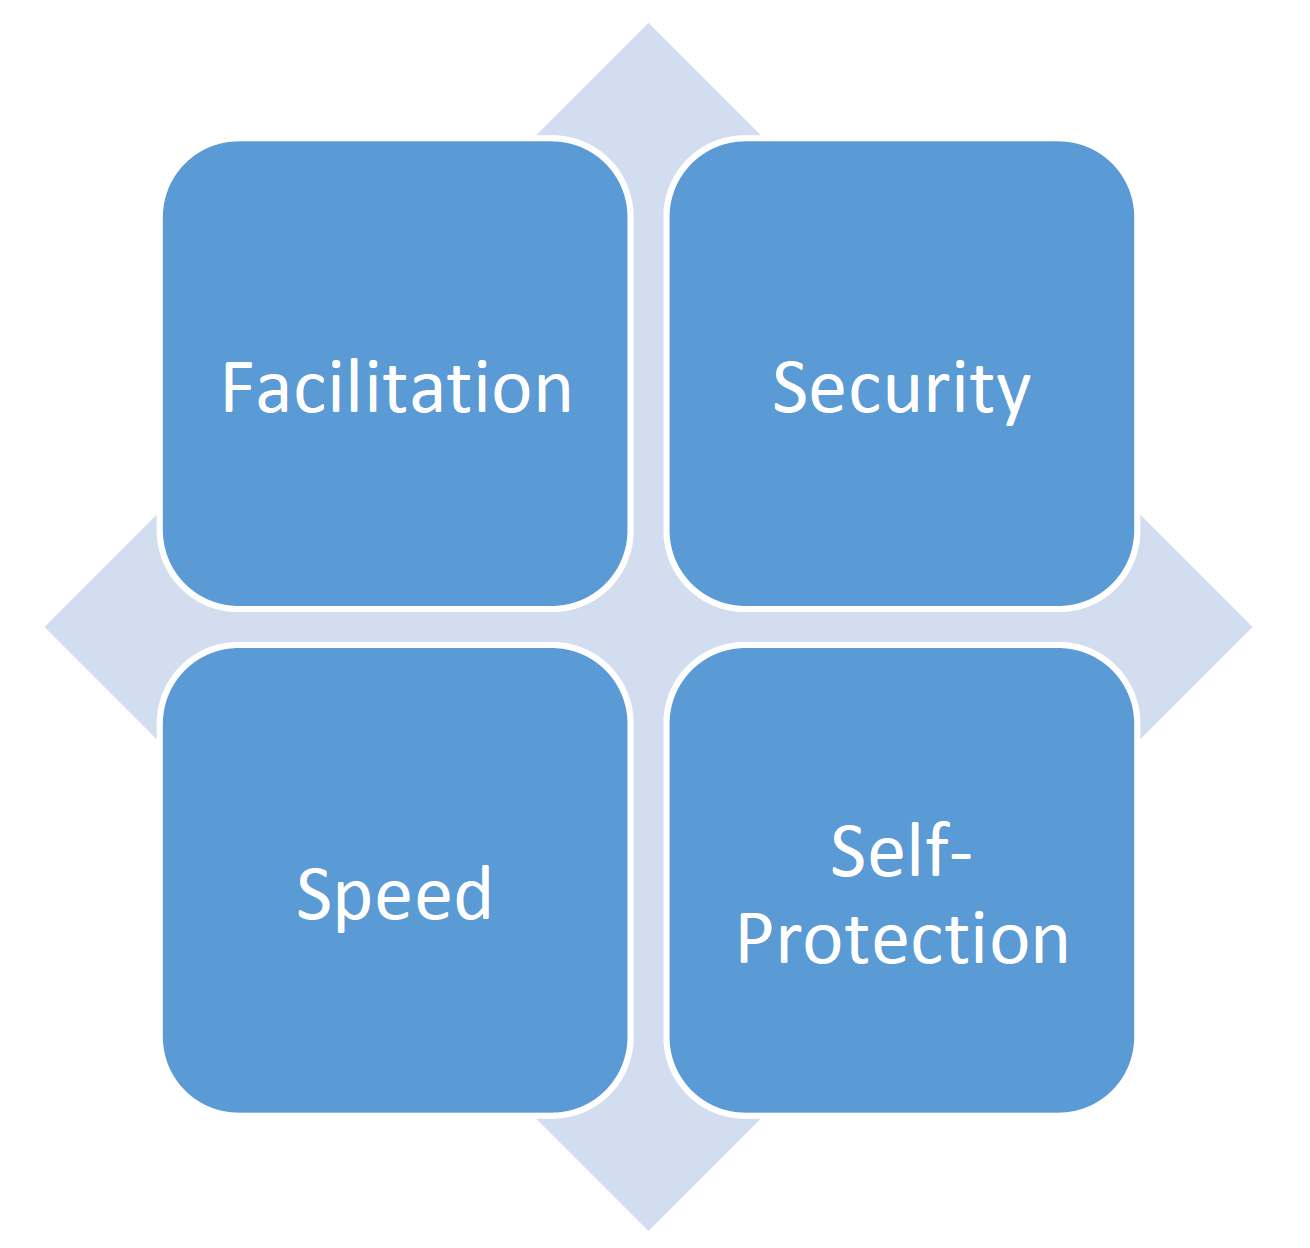
\includegraphics[height=5.2cm]{Figures/constraints}
	\caption{The operational constraints of the security agents.}
	\label{f:constraints}
\end{figure}



\subsubsection{ Error Types }


The security agents can usually do 3 types of error during the baggage inspection process.

\paragraph{Perception errors}:

The security agent does not detect the right area to analyze. He is not focus on the troublesome area, see figure \ref{f:perception}.
\begin{figure}
\centering
	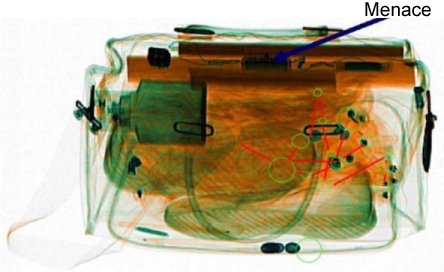
\includegraphics[height=8cm]{Figures/perceptionError}
	\caption{Perception error. The security agent do not notice the menace at the top of the image (the initiating system of an explosive) }
	\label{f:perception}
\end{figure}
\paragraph{Interpretation errors}:

The security agent detects the right troublesome area but does not judge it as a potential threat. In other words, he is focused on the right area but cannot see the menace. The agents used to combine what they find out with their knowledge on real world objects stored in their memories. They have their own model of the situation, see figure \ref{f:interpretation}.
\begin{figure}
\centering
	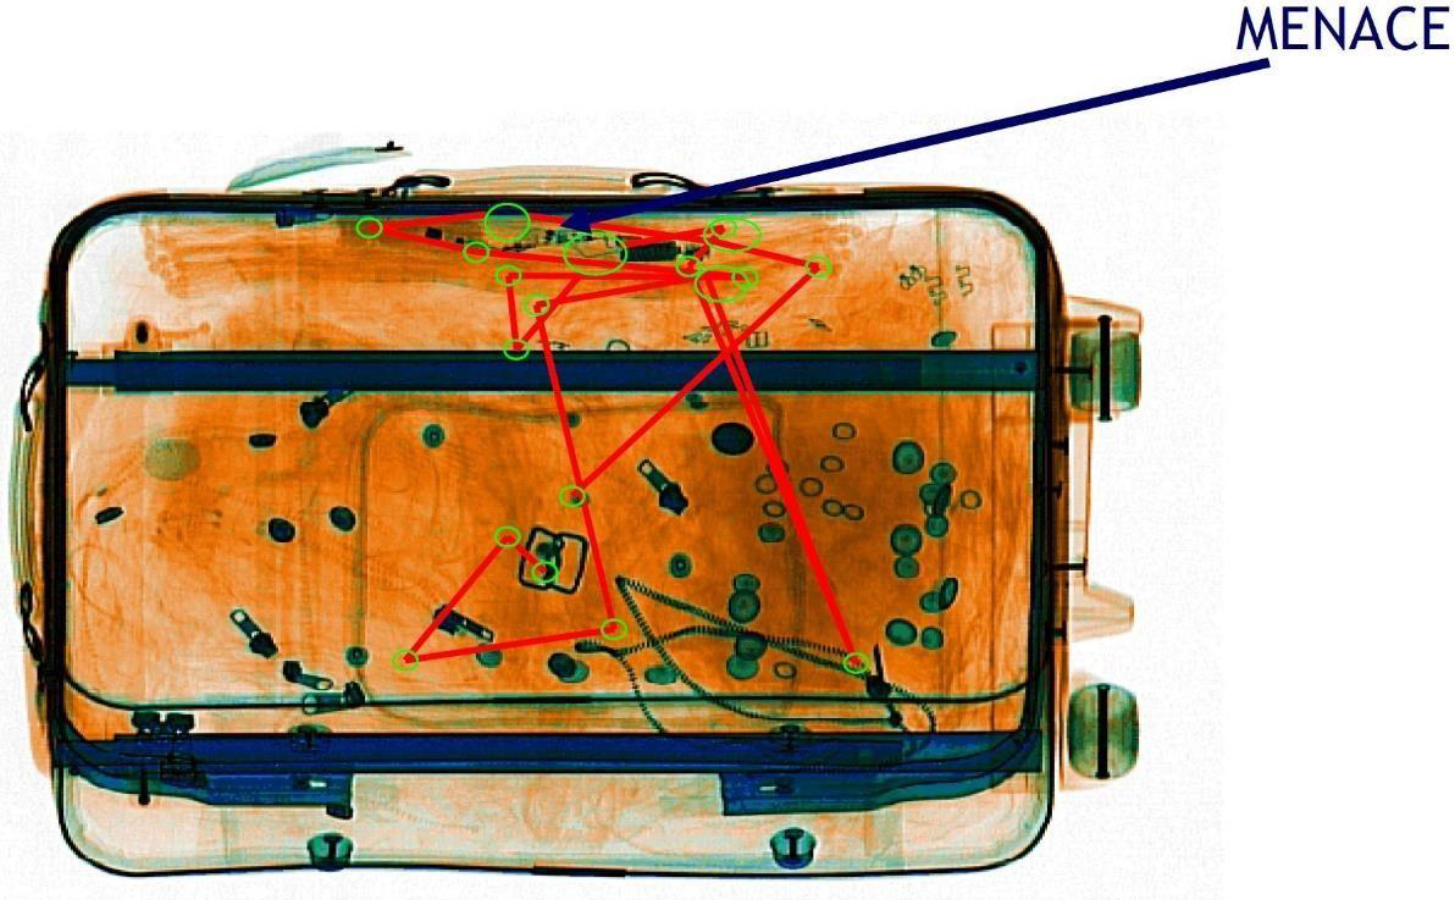
\includegraphics[height=8cm]{Figures/interpretationError}
	\caption{Interpretation errors. The security agent notice the menace at the top of the image do not interpret it as a threat (the initiating system of an explosive)}
	\label{f:interpretation}
\end{figure}

\paragraph{Decision making errors}:
In this case, the security agent detects the right troublesome area with a good interpretation, but make a bad decision. It might be related to the context or the procedure knowledge.
In addition to these errors related to the agent, four hiding techniques can be used to bypass the security mechanisms. Those techniques are superposition, positioning, dissociation, and bait.

\subsubsection{ Dissimulation techniques }
Since the resulting X-ray scanned image only contains densities, it cannot display the material original colors. The standard color visual mapping uses 3 different colors (orange, green, and blue) to display the data density. Orange color corresponds to low density (mainly organic items). In opposition, blue color is used for high density items (e.g. metal). In the case of X-ray systems, green color corresponds to the superposition of different kinds of materials or average density materials (\ref{f:image2d}). 

The displayed 2D scanned image can suffer from four issues.

\textbf{Superposition}: A threat (e.g. prohibited object like knife, cutter…) may be sheltered behind dense materials. Sometimes, it is possible to see through these blind shield using some functionalities such as high penetration (enhanced X-ray power) or image processing (contrast improvement),  see figure \ref{f:superposition}. 
\begin{figure}
\centering
	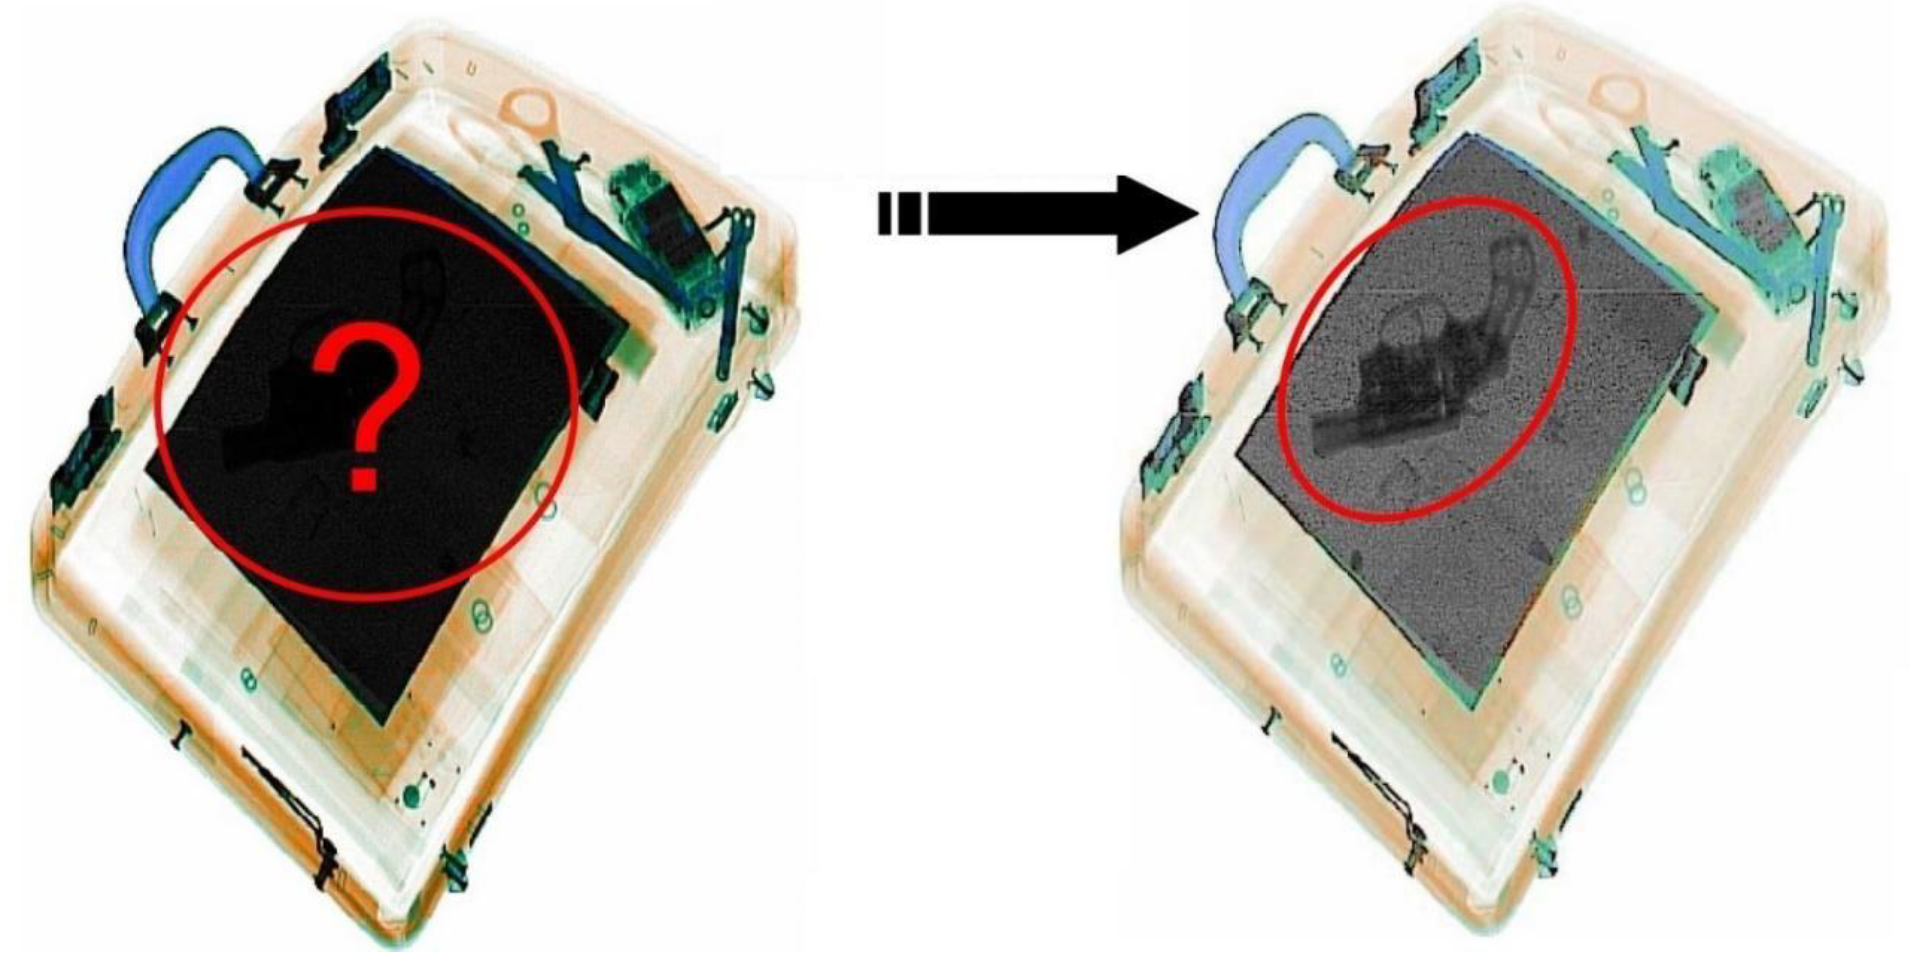
\includegraphics[height=8cm]{Figures/superposition}
	\caption{Dissimulation by superposition}
	\label{f:superposition}
\end{figure}

\textbf{Location}: Depending on its location inside the luggage, a threat can be difficult to detect. Objects located in the corners, in the edges or inside the luggage's frame are very difficult to identify,  see figure \ref{f:location}.
\begin{figure}
\centering
	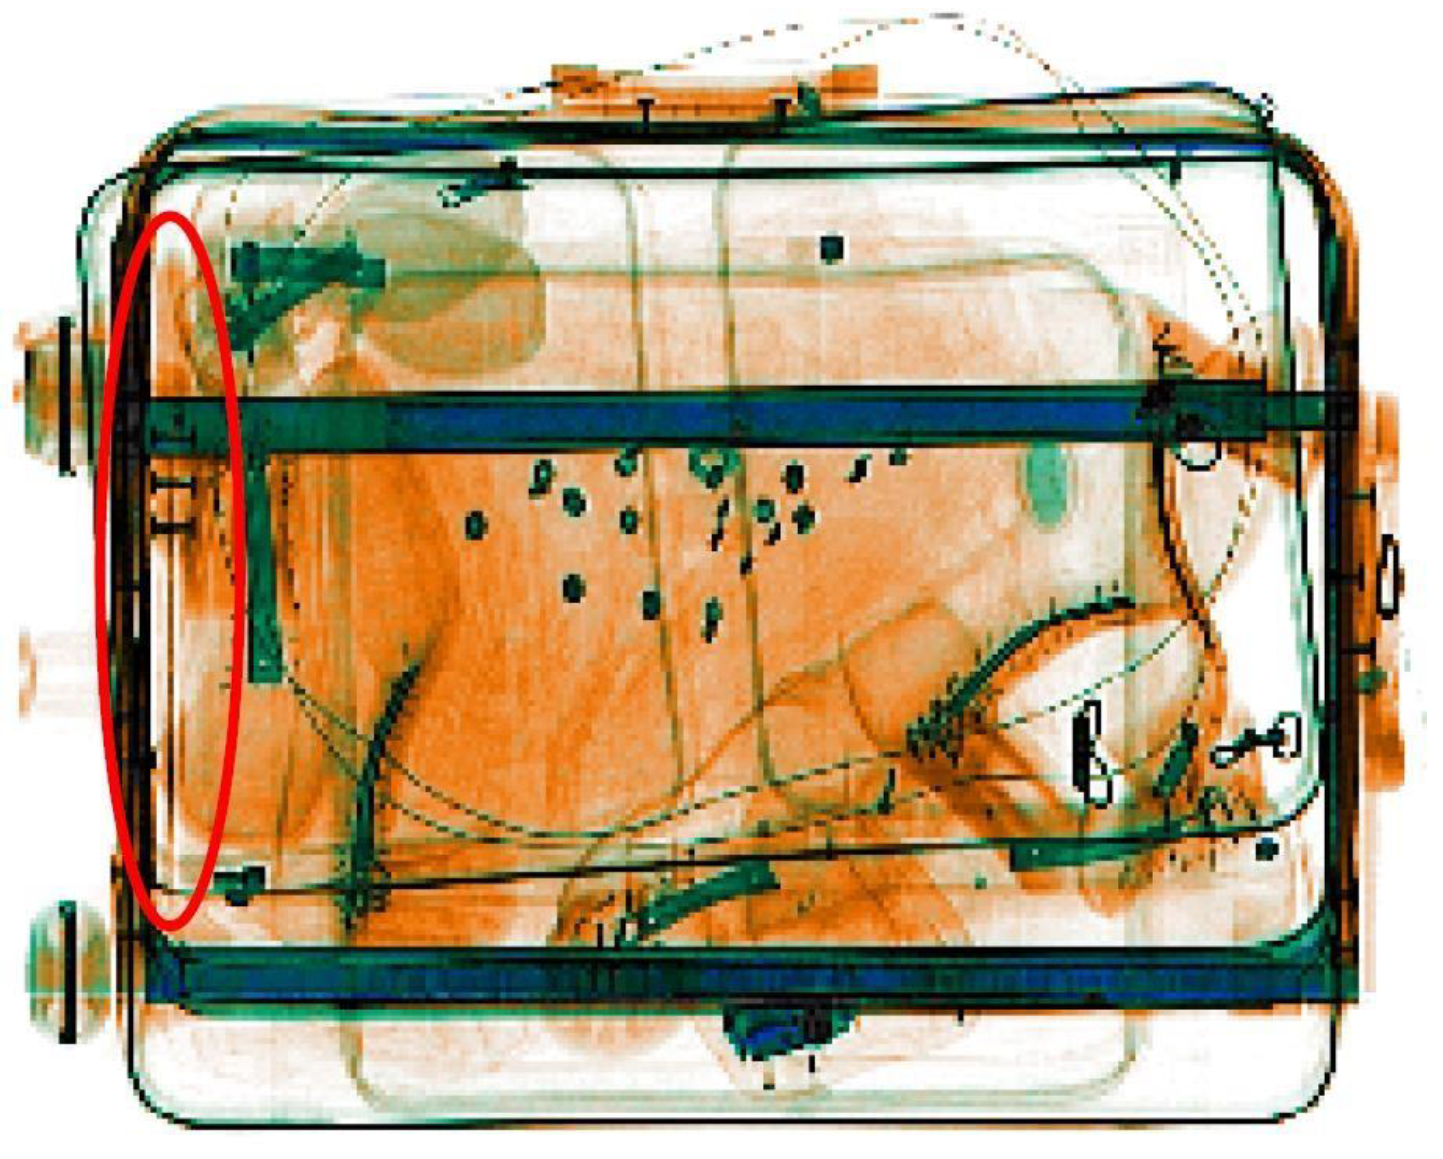
\includegraphics[height=8cm]{Figures/positioning}
	\caption{Dissimulation by the location}
	\label{f:location}
\end{figure}

\textbf{Dissociation}: Another way to dissimulate a threat is to separate and to spread parts of it in the luggage (weapon or explosive are composed of many separated items like the trigger, the cannon...). This dissociation can be combined with other dissimulation techniques,  see figure \ref{f:dissociation}.
\begin{figure}
\centering
	\includegraphics[height=8cm]{Figures/Dissociation}
	\caption{Dissimulation by dissociation}
	\label{f:dissociation}
\end{figure}

\textbf{Lure}: An ill-intentioned individual may use a lure to hide the real threat. For instance, a minor threat like a small scissors may be clearly visible and catch security agent's attention while a more important threat remains hidden, see figure \ref{f:bait}.
\begin{figure}
\centering
	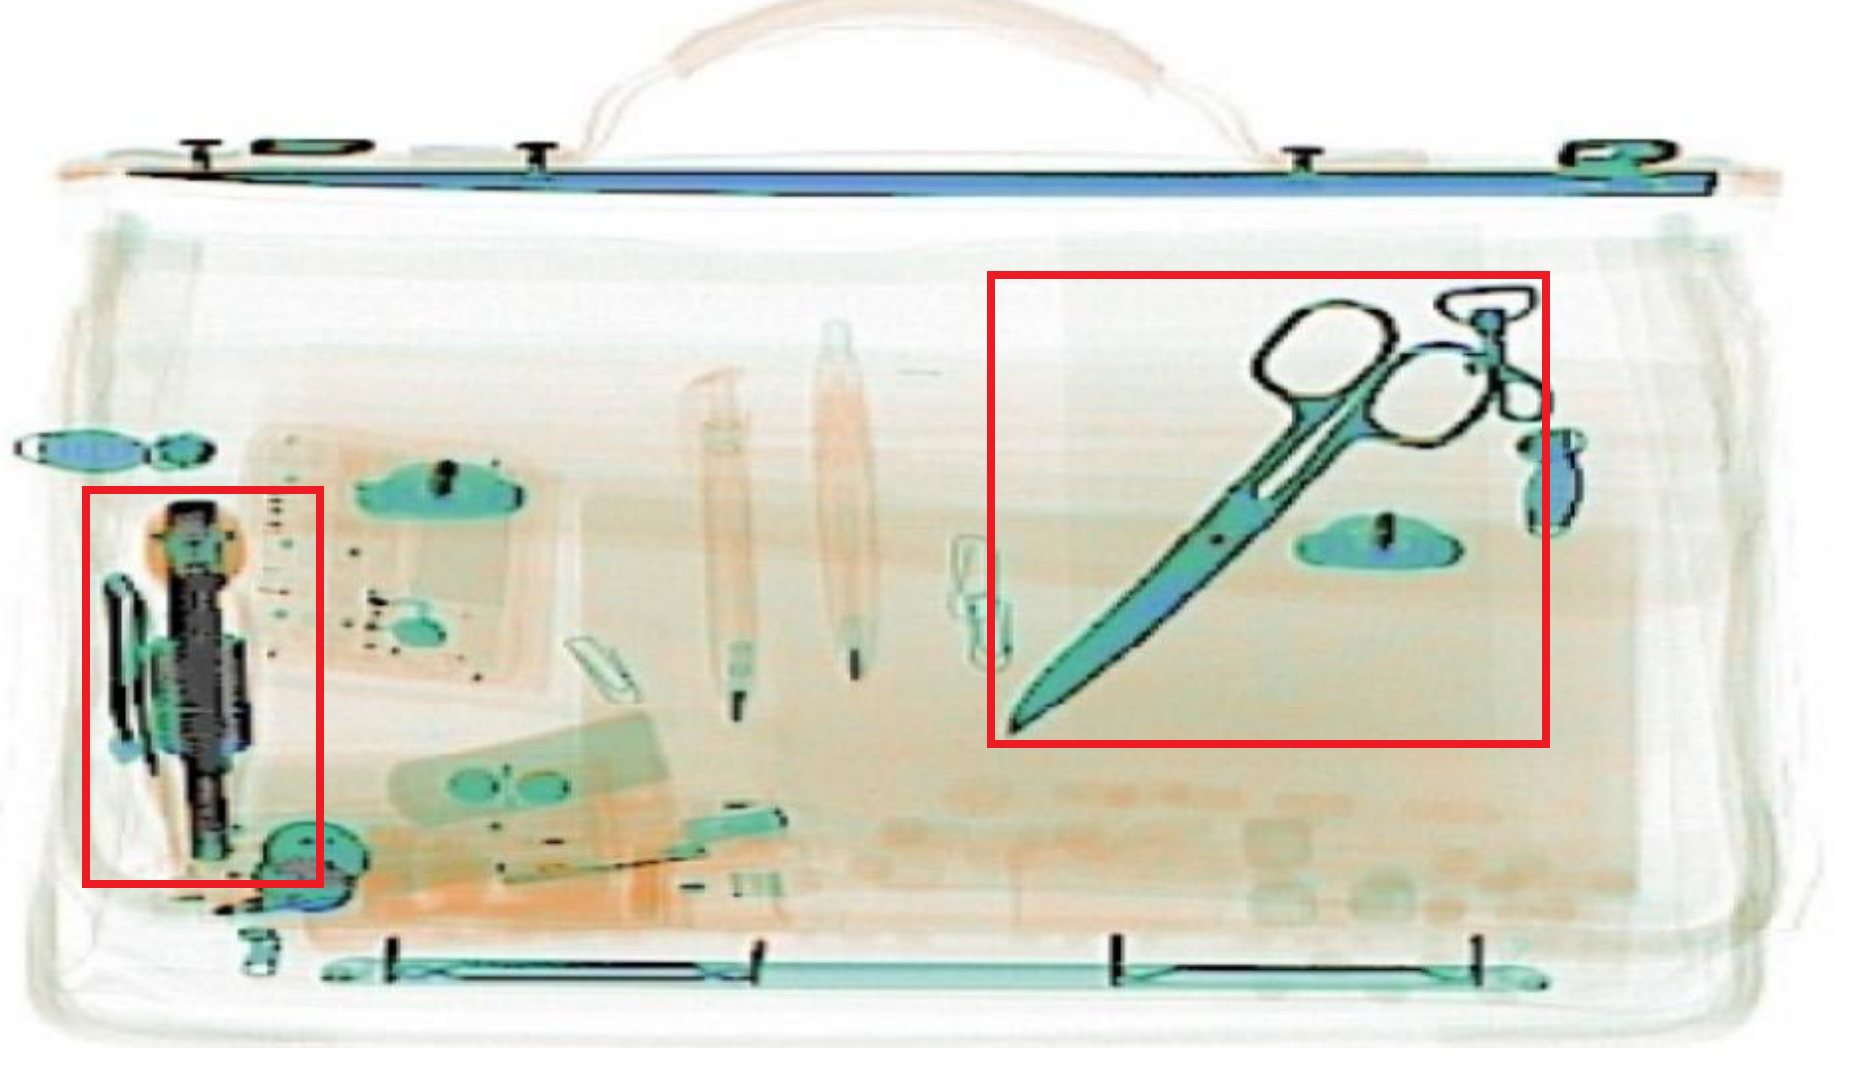
\includegraphics[height=8cm]{Figures/bait}
	\caption{Dissimulation using a bait}
	\label{f:bait}
\end{figure}

\subsection{ Requirements }


3D baggage scan exploration are one potential solution of such limitations, but to the best of our knowledge no previous existing system investigated this activity domain with interactive volumetric exploration tools. Even if extensive works have been done in medical 3D scan exploration and manipulation ~\cite{preim2013visual}, there is a great opportunity to adapt and develop new interaction and data manipulation techniques to support 3D baggage exploration.

We performed on site observations with contextual inquiry (one day observation in one of the major French airport). We also conducted one brainstorming with four security practitioners from which we defined relevant use cases. Thanks to these analysis, we extracted a set of top level needs and requirements :

•	VIS: users need to visualize the content of the luggage.

•	EXP: users have to explore the baggage with interactive navigation system.

•	OCL: the system must provide tools to address occlusion issues; the
superposition of items inside the luggage hinders their visualization.

•	INT: User need to explore luggage with simple interactions. User knowledge is too limited regarding volumetric data processing to understand the involved techniques and their parameters.

\section{ Interactive exploration of 3D scanned baggage }

\subsection{Top Level Structure}

Our system is composed of one main view (Volume Visualization) and 5 sub views to control and customize it, see figure \ref{f:layout}. Our interactive system does not provide menu and every feature is directly accessible from this main view (\autoref{f:figure2}).
The Volume Visualization can contain up to two views to ease interactions with the 3D scan. These views display the baggage and one can navigate through it (zoom, pan, rotation), manipulate its content (brushing, selection, deletion). These two views can be linked or disconnected in order to inspect selected objects with or without their context.
A smaller view called Overview shows the location of the investigated area. The overview is one-eighth the size of the main window and is located at its bottom right.
\begin{figure}
\centering
	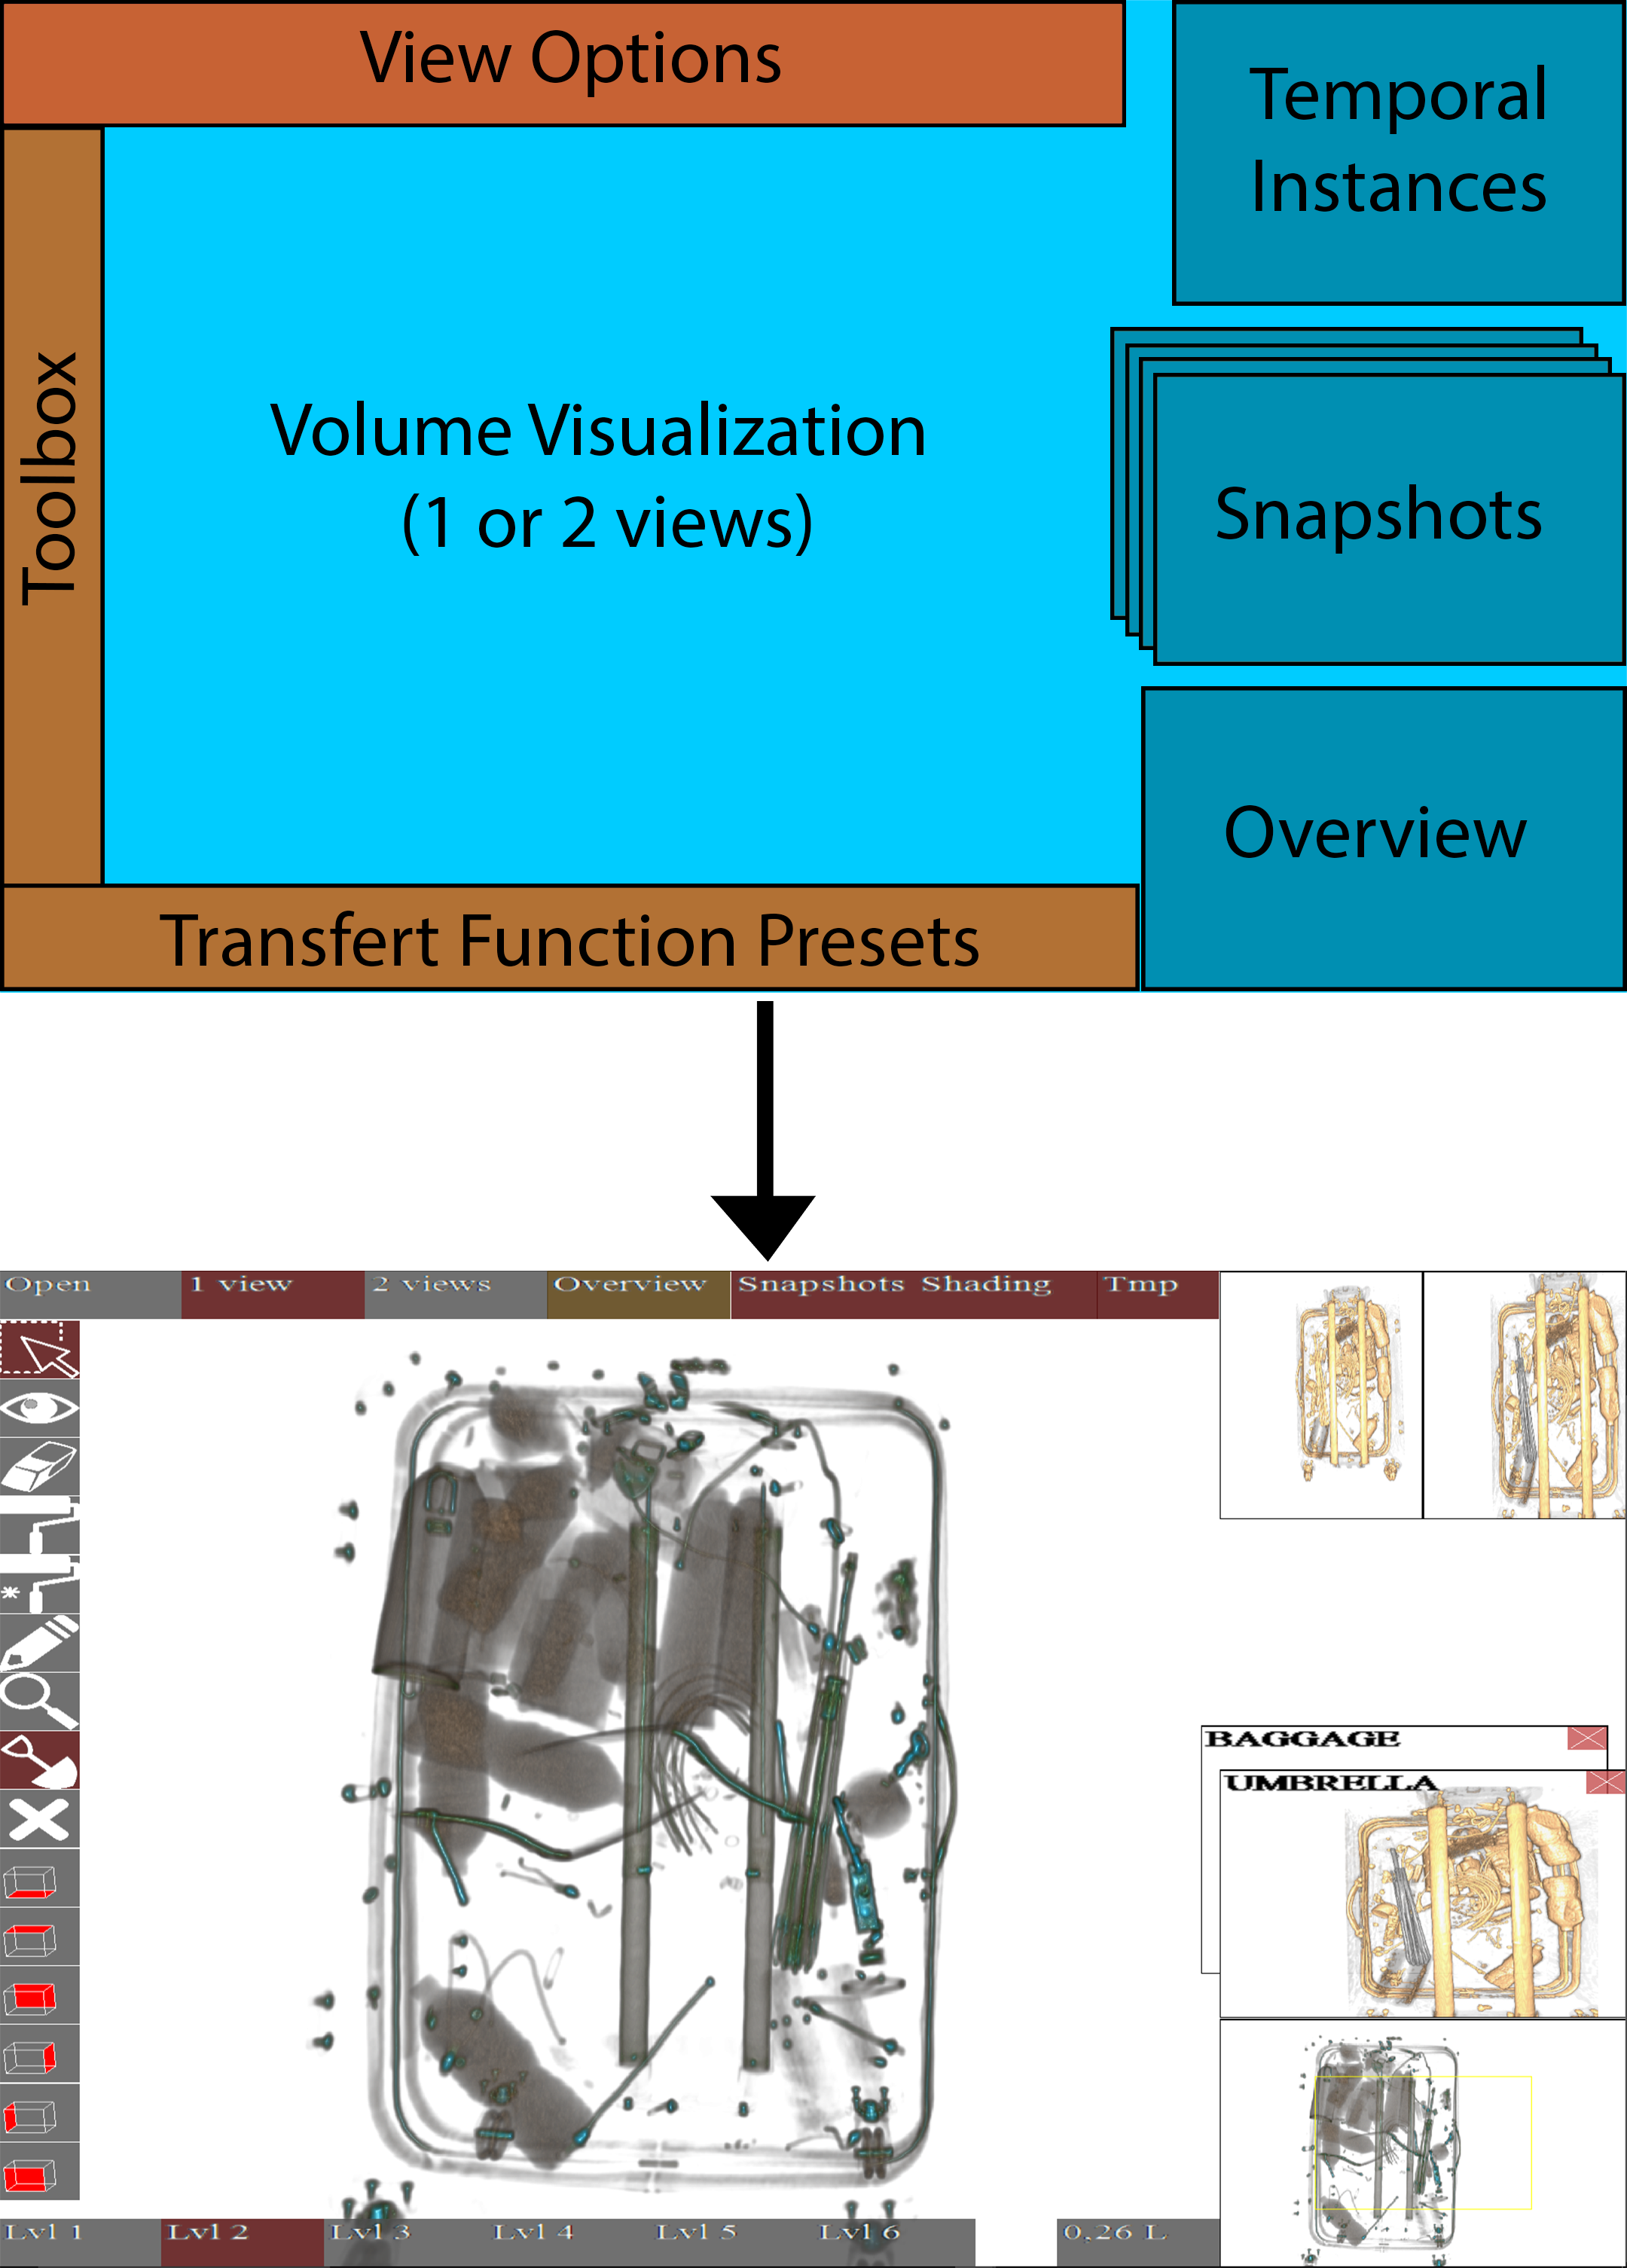
\includegraphics[height=14cm]{Figures/layout}
	\caption{Top level layout and screenshot of our Graphical User Interface. All the features are available throught this GUI}
	\label{f:layout}
\end{figure}

Temporal Instances window, located in the top right of the interface, shows the current and the previous settings of the Volume Visualization. The current setting is modified when the user changes the transfer function or manipulates an object.
The Snapshot shows saved instances with their setting (pan, zoom, rotation, transfer function, selection, brushing).
The Toolbox contains every interactive tools to explore the baggage (brushing, selection, eraser, density picker, navigation tools).
Transfer Function presets contains six predefined settings ordered by their filtering power. Low level shows every density, high level only show high density values. 
This global layout can be customized thanks to View Options. One can display one or two views of the Volume Visualization, the Temporal Instances, the Snapshot and the Overview.